%%%%%%%%%%%%%%%%%%%%%%%%%%%%%%%%%%%%%%%%%
% Programming/Coding Assignment
% LaTeX Template
%
% This template has been downloaded from:
% http://www.latextemplates.com
%
% Original author:
% Ted Pavlic (http://www.tedpavlic.com)
%
% Note:
% The \lipsum[#] commands throughout this template generate dummy text
% to fill the template out. These commands should all be removed when 
% writing assignment content.
%
% This template uses a Perl script as an example snippet of code, most other
% languages are also usable. Configure them in the "CODE INCLUSION 
% CONFIGURATION" section.
%
%%%%%%%%%%%%%%%%%%%%%%%%%%%%%%%%%%%%%%%%%

%----------------------------------------------------------------------------------------
%	PACKAGES AND OTHER DOCUMENT CONFIGURATIONS
%----------------------------------------------------------------------------------------

%\documentclass{article}
\documentclass[12pt]{article}
\usepackage{fancyhdr} % Required for custom headers
\usepackage{lastpage} % Required to determine the last page for the footer
\usepackage{extramarks} % Required for headers and footers
\usepackage[usenames,dvipsnames]{color} % Required for custom colors
\usepackage{graphicx} % Required to insert images
\usepackage{subcaption}
\usepackage{listings} % Required for insertion of code
\usepackage{courier} % Required for the courier font
\usepackage{amsmath}
\usepackage{framed}

% Margins
\topmargin=-0.45in
\evensidemargin=0in
\oddsidemargin=0in
\textwidth=6.5in
\textheight=9.0in
\headsep=0.25in

\linespread{1.1} % Line spacing

% Set up the header and footer
\pagestyle{fancy}
\lhead{\hmwkAuthorName} % Top left header
\chead{\hmwkClass\ (\hmwkClassTime): \hmwkTitle} % Top center head
%\rhead{\firstxmark} % Top right header
\lfoot{\lastxmark} % Bottom left footer
\cfoot{} % Bottom center footer
\rfoot{Page\ \thepage\ of\ \protect\pageref{LastPage}} % Bottom right footer
\renewcommand\headrulewidth{0.4pt} % Size of the header rule
\renewcommand\footrulewidth{0.4pt} % Size of the footer rule

\setlength\parindent{0pt} % Removes all indentation from paragraphs

%----------------------------------------------------------------------------------------
%	CODE INCLUSION CONFIGURATION
%----------------------------------------------------------------------------------------

\definecolor{mygreen}{rgb}{0,0.6,0}
\definecolor{mygray}{rgb}{0.5,0.5,0.5}
\definecolor{mymauve}{rgb}{0.58,0,0.82}

\lstset{ %
  backgroundcolor=\color{white},   % choose the background color
  basicstyle=\footnotesize,        % size of fonts used for the code
  breaklines=true,                 % automatic line breaking only at whitespace
  captionpos=b,                    % sets the caption-position to bottom
  commentstyle=\color{mygreen},    % comment style
  escapeinside={\%*}{*)},          % if you want to add LaTeX within your code
  keywordstyle=\color{blue},       % keyword style
  stringstyle=\color{mymauve},     % string literal style
}

%----------------------------------------------------------------------------------------
%	DOCUMENT STRUCTURE COMMANDS
%	Skip this unless you know what you're doing
%----------------------------------------------------------------------------------------

% Header and footer for when a page split occurs within a problem environment
\newcommand{\enterProblemHeader}[1]{
%\nobreak\extramarks{#1}{#1 continued on next page\ldots}\nobreak
%\nobreak\extramarks{#1 (continued)}{#1 continued on next page\ldots}\nobreak
}

% Header and footer for when a page split occurs between problem environments
\newcommand{\exitProblemHeader}[1]{
%\nobreak\extramarks{#1 (continued)}{#1 continued on next page\ldots}\nobreak
%\nobreak\extramarks{#1}{}\nobreak
}

\setcounter{secnumdepth}{0} % Removes default section numbers
\newcounter{homeworkProblemCounter} % Creates a counter to keep track of the number of problems
\setcounter{homeworkProblemCounter}{0}

\newcommand{\homeworkProblemName}{}
\newenvironment{homeworkProblem}[1][Part \arabic{homeworkProblemCounter}]{ % Makes a new environment called homeworkProblem which takes 1 argument (custom name) but the default is "Problem #"
\stepcounter{homeworkProblemCounter} % Increase counter for number of problems
\renewcommand{\homeworkProblemName}{#1} % Assign \homeworkProblemName the name of the problem
\section{\homeworkProblemName} % Make a section in the document with the custom problem count
\enterProblemHeader{\homeworkProblemName} % Header and footer within the environment
}{
\exitProblemHeader{\homeworkProblemName} % Header and footer after the environment
}

\newcommand{\problemAnswer}[1]{ % Defines the problem answer command with the content as the only argument
\noindent\framebox[\columnwidth][c]{\begin{minipage}{0.98\columnwidth}#1\end{minipage}} % Makes the box around the problem answer and puts the content inside
}

\newcommand{\homeworkSectionName}{}
\newenvironment{homeworkSection}[1]{ % New environment for sections within homework problems, takes 1 argument - the name of the section
\renewcommand{\homeworkSectionName}{#1} % Assign \homeworkSectionName to the name of the section from the environment argument
\subsection{\homeworkSectionName} % Make a subsection with the custom name of the subsection
\enterProblemHeader{\homeworkProblemName\ [\homeworkSectionName]} % Header and footer within the environment
}{
\enterProblemHeader{\homeworkProblemName} % Header and footer after the environment
}

%----------------------------------------------------------------------------------------
%	NAME AND CLASS SECTION
%----------------------------------------------------------------------------------------

\newcommand{\hmwkTitle}{Assignment 1} % Assignment title
\newcommand{\hmwkDueDate}{Thrusday, Jan 31, 2019} % Due date
\newcommand{\hmwkClass}{CSC421} % Course/class
\newcommand{\hmwkClassTime}{LEC 5101} % Class/lecture time
\newcommand{\hmwkAuthorName}{Zhongtian Ouyang} % Your name
\newcommand{\hmwkAuthorID}{1002341012} % Your ID


%----------------------------------------------------------------------------------------
%	TITLE PAGE
%----------------------------------------------------------------------------------------

\title{
\vspace{2in}
\textmd{\textbf{\hmwkClass:\ \hmwkTitle}}\\
\normalsize\vspace{0.1in}\small{Due\ on\ \hmwkDueDate}\\
\vspace{0.1in}
\vspace{3in}
}

\author{\textbf{\hmwkAuthorName}\\ \textbf{\hmwkAuthorID}}

\date{} % Insert date here if you want it to appear below your name

%----------------------------------------------------------------------------------------\
\begin{document}

\maketitle
\clearpage

%----------------------------------------------------------------------------------------
%	Common Tools
%----------------------------------------------------------------------------------------
%\begin{framed}
%\begin{lstlisting}[language=matlab]
%\end{lstlisting}
%\end{framed}

% \begin{bmatrix}
%0.5 & 0.6 \\ 
%0.7 & 0.8
%\end{bmatrix}

%\begin{figure}[h!]
%\centering
%\includegraphics[width=0.6\linewidth]{q10a.png}
%\label{fig:q10a}
%\end{figure}\\

%\begin{figure*}[!ht]
%\begin{subfigure}{.5\textwidth}
% \centering
%  \includegraphics[width=.5\linewidth]{p4_1.JPG}
%  \caption{Full set}
%  \label{fig:sfig1}
%\end{subfigure}
%\begin{subfigure}{.5\textwidth}
% \centering
%  \includegraphics[width=.5\linewidth]{P4_2.JPG}
%  \caption{Two each}
%  \label{fig:sfig2}
%\end{subfigure}%
%\caption{Part4 (a)}
%\label{fig:p4a}
%\end{figure*}

%\sum_{n=1}^{\infty} 2^{-n} = 1
%\prod_{i=a}^{b} f(i)
%----------------------------------------------------------------------------------------
%	PROBLEM 1
%----------------------------------------------------------------------------------------

% To have just one problem per page, simply put a \clearpage after each problem
\begin{homeworkProblem}
1.\\
word\_embedding\_weights: $250 \times 16 = 4000$\\
embed\_to\_hid\_weights: $(16 \times 3) \times 128 = 6144$\\
hid\_bias: $128$\\
hid\_to\_output\_weights: $128 \times 250 = 32000$\\
output\_bias: $250$\\
We can see that we have $4000 + 6144 + 128 + 32000 + 250 = 42522$ trainable parameters\\
hid\_to\_output\_weights has the largest number of trainable parameters.\\

2.\\
In a 4-gram model, each word position has 250 possible choices. We need $250^4 = 3,906,250,000$ entries to store the counts of all possible 4-grams explicitly.
\end{homeworkProblem}
%----------------------------------------------------------------------------------------
%	PROBLEM 2
%----------------------------------------------------------------------------------------

\begin{homeworkProblem}
\begin{framed}
\begin{lstlisting}[language=python]
loss_derivative[2, 5] 0.001112231773782498
loss_derivative[2, 121] -0.9991004720395987
loss_derivative[5, 33] 0.0001903237803173703
loss_derivative[5, 31] -0.7999757709589483

param_gradient.word_embedding_weights[27, 2] -0.27199539981936866
param_gradient.word_embedding_weights[43, 3] 0.8641722267354154
param_gradient.word_embedding_weights[22, 4] -0.2546730202374649
param_gradient.word_embedding_weights[2, 5] 0.0

param_gradient.embed_to_hid_weights[10, 2] -0.6526990313918255
param_gradient.embed_to_hid_weights[15, 3] -0.13106433000472612
param_gradient.embed_to_hid_weights[30, 9] 0.11846774618169396
param_gradient.embed_to_hid_weights[35, 21] -0.1000452610460439

param_gradient.hid_bias[10] 0.2537663873815642
param_gradient.hid_bias[20] -0.03326739163635368

param_gradient.output_bias[0] -2.0627596032173052
param_gradient.output_bias[1] 0.0390200857392169
param_gradient.output_bias[2] -0.7561537928318482
param_gradient.output_bias[3] 0.21235172051123635
\end{lstlisting}
\end{framed}

\end{homeworkProblem}
\clearpage
%----------------------------------------------------------------------------------------
%	PROBLEM 3
%----------------------------------------------------------------------------------------

\begin{homeworkProblem}
1.\\
The three-word phrase I pick is ``he is the''. I get the following result from model:\\
he is the best Prob: 0.23524\\
he is the same Prob: 0.10197\\
he is the only Prob: 0.07203\\
he is the first Prob: 0.05316\\
he is the right Prob: 0.04734\\
he is the last Prob: 0.03425\\
he is the other Prob: 0.03199\\
he is the people Prob: 0.03023\\
he is the case Prob: 0.02653\\
he is the end Prob: 0.02199\\
All these predictions seems to be sensible. Among these predictions, ``he is the right'', ``he is the last'', ``he is the other'', ``he is the people'', ``he is the case'' and ``he is the end'' weren't present in the dataset, and all these 4-grams seems plausible, especially ``he is the right'', ``he is the last'', ``he is the other''.\\

2.\\
(should, might, may, would, could, can, will) is a cluster of words. We can see the usage of these words are very similar. They appears in the same position of a sentence with somewhat similar meanings.\\
(how, when, who, where, what) is a cluster of words. These words are all used as part of a question.\\
(does, do, did) and (be, been, was, is, were, are) are two clusters of words. Words in the first cluster are different tenses of ``do'' while words in the second cluster are different tenses of ``be''.\\

3.\\
The word distance for ``new'' and ``york'' is 3.57. And from the tsne graph, we can see that they are not really close to each other. The reason is that even though the phrase ``new york'' appears a lot, ``new'' and ``york'' have different functions. The word ``new'' is also used a lot as a adjective describing items, while ``york'' can't be used like that.\\

4.\\
The word distance for ``government'' and ``university'' is 1.044 while the word distance for ``government'' and ``political'' is 1.376. It is obvious that (government, university) is closer together. The reason could be that even though ``government'' and ``policical'' have related meanings, ``government'' and ``university'' have closer encodings because they are both nouns and types of organizations. They appear in similar positions of a sentence. \\

\begin{figure}[h!]
\centering
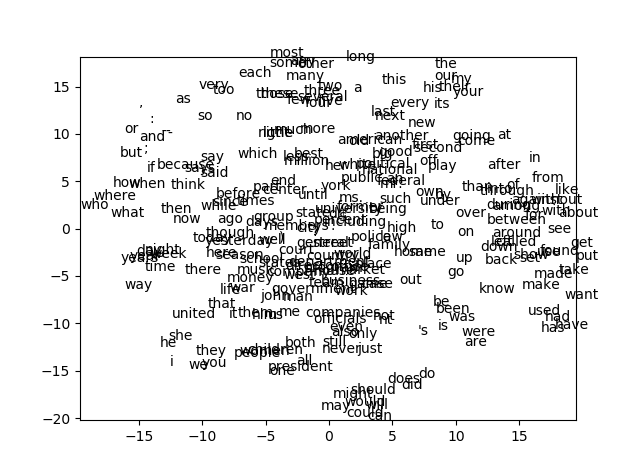
\includegraphics[width=\linewidth]{Figure_1.png}
\caption{TSNE Graph}
\end{figure}
\end{homeworkProblem}
%----------------------------------------------------------------------------------------

\end{document}
